\chapter{System Overview [AS PER FYP1 MID REPORT]}

\textbf{ForeSyte} AI Exam Surveillance System is an intelligent monitoring solution designed to enhance the integrity of in-person examinations by automating student and invigilator monitoring. The system integrates CCTV cameras, computer vision, and deep learning models to detect suspicious student behaviors such as phone usage, frequent seat movements, or unauthorized communication, while also tracking invigilator activities to ensure accountability. Each activity is mapped to seating plans to ensure accurate identification of students. Detected events are logged as timestamped violations, which are compiled into structured reports accessible through an administrative dashboard. Administrators manage user profiles, seating plans, and exam sessions, while disciplinary investigators utilize the violation reports to review cases and make informed decisions. The system follows a modular architecture consisting of two primary components: the ForeSyte Web Portal, a multi-user web interface for dashboard visualization and report management, and the Backend Service, the core AI engine handling video stream processing, cheating detection, seat mapping, and automated report generation. This architectural design ensures separation of concerns, scalability, and maintainability while providing seamless integration between the user interface and the underlying AI processing capabilities.

\section{Architectural Design}

The ForeSyte AI Exam Surveillance System is designed using a modular architecture to ensure scalability, maintainability, and clear separation of concerns. At a high level, the system is divided into front-end modules, back-end modules, and supporting external systems. Each module plays a distinct role but collaborates with others to achieve the overall goal of automated, AI-powered exam monitoring.

The architecture follows a \textbf{two-tier client-server architecture} with \textbf{layered components}, implementing a \textbf{RESTful API} design pattern. The front-end (presentation tier) handles user input, report visualization, and dashboard interactions through a React-based single-page application. The back-end (application tier) processes video streams, performs AI-based detection and analysis, and manages business logic through FastAPI routes. The data management layer (data tier) ensures persistence and retrieval of information using PostgreSQL for relational data and MongoDB for high-velocity event logs. This decomposition ensures that the AI detection logic, data storage, and user interfaces remain loosely coupled and independently upgradable.

\subsection{Box and Line Diagram (Initial Design Stage)}
In the initial design stage, a simple box and line diagram is used to represent the main system components and their interactions. This diagram provides a high-level overview of how the core modules connect, without detailing the internal architecture or data flow.

\begin{figure}[H]
    \centering
    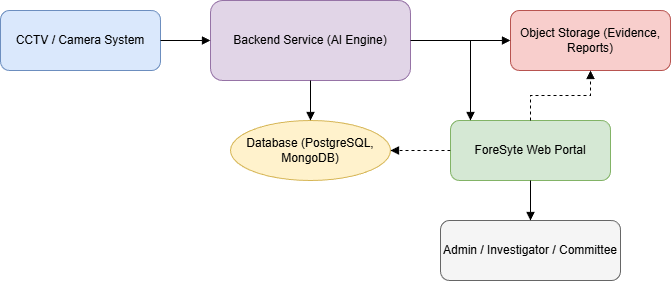
\includegraphics[width=0.85\textwidth]{sections/box-line.drawio.png}
    \caption{Box and Line Diagram for ForeSyte AI Exam Surveillance System}
    \label{fig:box-line}
\end{figure}
\FloatBarrier

\subsection{High-Level Architectural Style}
After the initial overview, the finalized architecture style/pattern diagram is presented. The system uses a two-tier client-server architecture with layered components, providing clear separation between the presentation layer (React frontend), application layer (FastAPI backend with embedded business logic), and data management layer (PostgreSQL and MongoDB). Figure~\ref{fig:architecture} illustrates the high-level architecture of the system, showing the main subsystems and their interactions.

\begin{figure}[H]
    \centering
    \caption{High-Level Architectural Design of the ForeSyte AI Exam Surveillance System}
    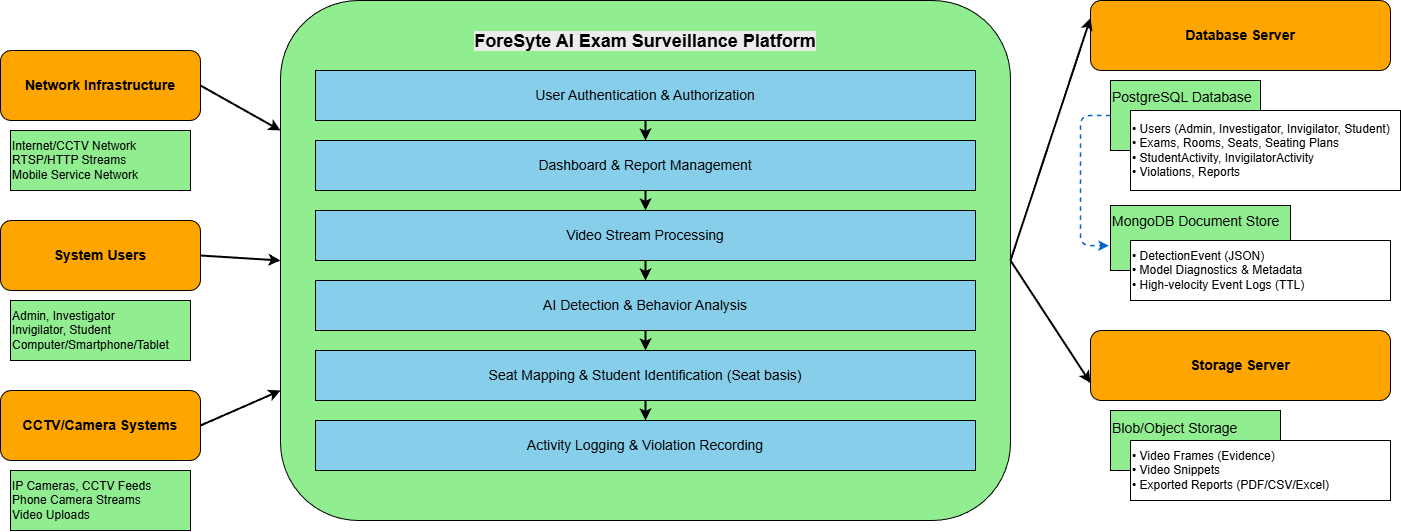
\includegraphics[width=\textwidth]{sections/foresyte-architecture-style.drawio.png}
    \label{fig:architecture}
\end{figure}
\FloatBarrier

\subsection{Mapping of Modules/Components}
Each module/component is mapped to its respective part of the architecture, ensuring modularity and scalability. The architecture supports integration with external systems (CCTV, storage, databases) and provides a robust foundation for AI-powered exam monitoring.

\section{Data Design}

The data design for \textbf{ForeSyte} focuses on how the system's information domain is represented and transformed into data structures across relational, document, and object stores. In this section, we outline the major system entities, how they are stored, processed, and managed to ensure robust operation and secure handling of user information and evidence.

\subsection{Data Structures and Organization}
ForeSyte deals with multiple data classes: user identities, seating plans, live/recorded video evidence, AI detections, activities, violations, and reports. The core data is organized so that:
\begin{itemize}
  \item \textbf{Relational (PostgreSQL)} holds normalized, queryable facts: Users, Exams, Rooms, Seats, StudentActivity, InvigilatorActivity, Violations, Reports, and seat assignments; enforced with foreign keys.
  \item \textbf{Document (MongoDB)} holds high-velocity \textit{DetectionEvent} JSON and model diagnostics with TTL, enabling fast ingest and optional replay/debug.
  \item \textbf{Blob/Object Storage} (evidence bucket) stores immutable artifacts: frame crops, video snippets, and exported PDF reports.
\end{itemize}

\paragraph{Data lifecycle.} Streams or uploads produce detection events; an aggregation service converts them into activities and violations with evidence links; dashboards and investigators read relational views and open the referenced evidence in object storage.

\subsection{Major Data Entities}
Key logical entities:
\begin{itemize}
  \item \textbf{User Information}: Admin, Invigilator, Investigator, and Student profiles with credentials and roles.
  \item \textbf{Exam/Room/Seat}: Exam sessions; rooms with cameras; seats mapped to students and exams.
  \item \textbf{DetectionEvent} (document): Raw detector output with timestamps, camera/room source, and model metadata.
  \item \textbf{StudentActivity/InvigilatorActivity}: Curated activities derived from detections; include severity, confidence, and optional evidence URL.
  \item \textbf{Violation}: Confirmed cheating events; include type, timestamp, severity, status, and optional evidence URL.
  \item \textbf{Report}: Generated summaries (PDF) of violations and activities for investigators.
\end{itemize}
\vspace{-0.5em} % ↓ Tightens space before the next heading

\subsection{Data Flow Diagrams (DFDs)}
\vspace{-0.25em} % ↓ Minimizes gap under heading

This subsection presents the logical data flow within the ForeSyte system at two abstraction levels.
Level 0 provides an overview of the main system interactions, while Level 1 elaborates on internal data processing — especially how seat mapping, activity detection, and behavior monitoring are interconnected.

\paragraph{Level 0 – Context Diagram}
Figure~\ref{fig:dfd-level0} illustrates the high-level data flow between external entities (such as Students, Invigilators, and Administrators) and the ForeSyte System. It highlights how examination footage, attendance data, and violation reports circulate through the system.

\begin{figure}[htbp]
    \centering
    \caption{DFD Level 0 – ForeSyte System Context Diagram}
    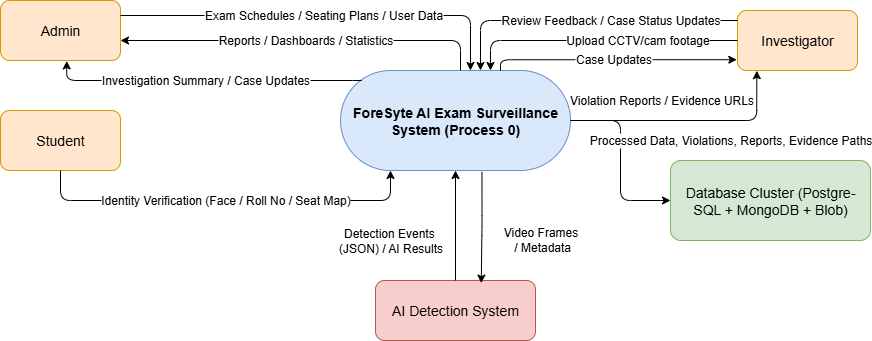
\includegraphics[width=\textwidth]{sections/DFD_Level0.drawio.png}
    \label{fig:dfd-level0}
\end{figure}


\paragraph{Level 1 – System Decomposition}
Figure~\ref{fig:dfd-level1} expands the ForeSyte process into its major internal modules: Seat Mapping, Cheating Detection Engine, Invigilator Monitoring, and Report Generation. Data from entry-point cameras are first processed to map activities to specific seats; this mapping is then propagated through subsequent modules for activity analysis and reporting.

\begin{figure}[htbp]
    \centering
    \caption{DFD Level 1 – Detailed ForeSyte System Data Flow}
    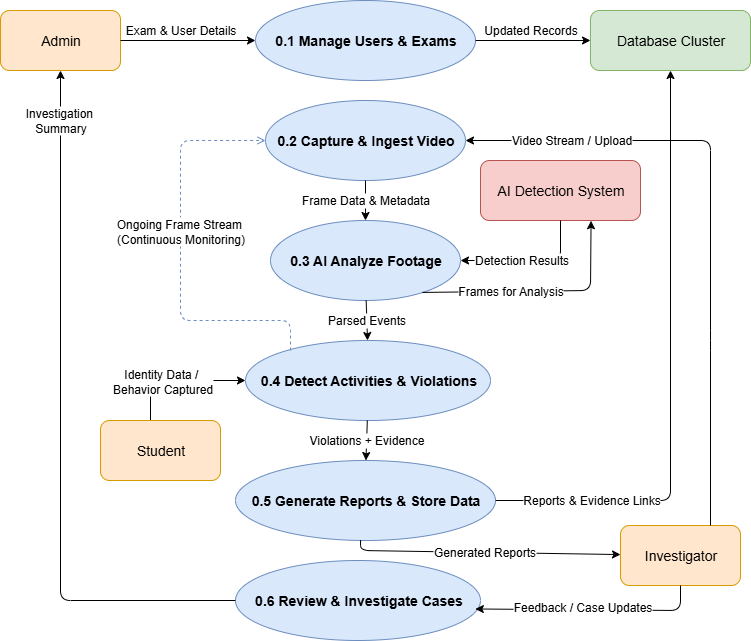
\includegraphics[width=\textwidth]{sections/DFD_Level1.drawio.png}
    \label{fig:dfd-level1}
\end{figure}
\clearpage


\subsection{Data Flow and Processing}
The system processes exam footage via two paths that converge into a unified pipeline:
\begin{enumerate}
  \item \textbf{Real-time (Live) Monitoring}: Camera streams feed the AI service, which emits per-frame \textit{DetectionEvents} (JSON).
  \item \textbf{Uploaded Footage}: After the exam, recorded video is ingested; the AI service produces the same \textit{DetectionEvents} offline.
  \item \textbf{Aggregation/Rules}: Business rules transform events into \textit{StudentActivity/InvigilatorActivity}; suspicious patterns yield \textit{Violation} rows with evidence links.
  \item \textbf{Persistence}: Normalized facts land in PostgreSQL; evidence media is stored in Blob/Object storage; optionally, transient raw events remain in MongoDB (TTL).
  \item \textbf{Consumption}: Admin dashboards query relational views; investigators open pre-signed evidence URLs and download reports.
\end{enumerate}
\let\cleardoublepage\clearpage
\section{Domain Model}
Figure \textcolor{blue}{\ref{fig:domain}} represents the domain model for ForeSyte. It outlines the key entities, their
attributes, and the relationships that define data interactions within the ForeSyte system.

\begin{figure}[htbp]
    \centering
    \caption{ForeSyte Domain Model Diagram}
    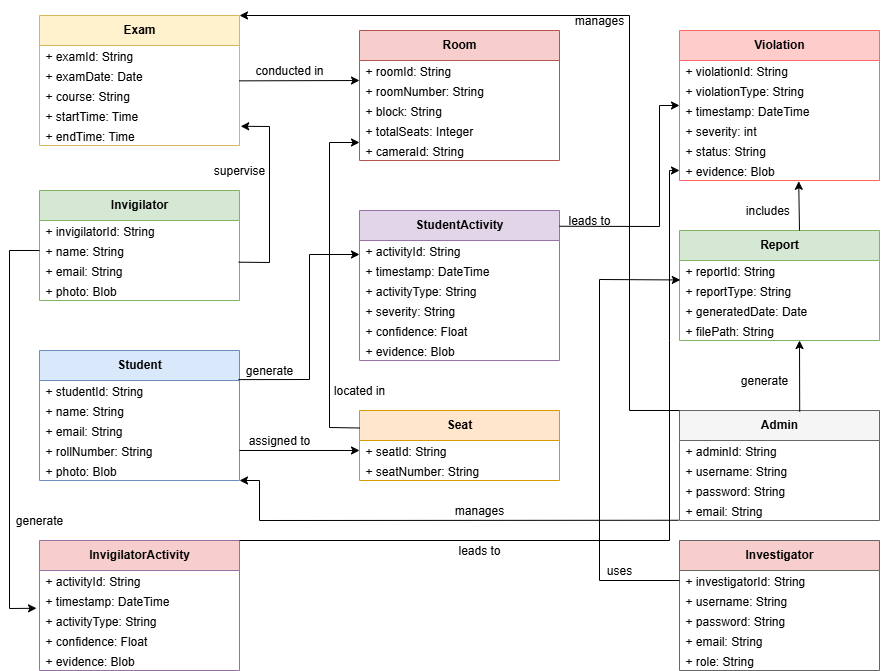
\includegraphics[width=\textwidth]{sections/domain-model.png}
    \label{fig:domain}
\end{figure}

\section{Design Models [UPTO THE CURRENT ITERATION ONLY]}

The ForeSyte system employs an object-oriented development approach, utilizing several key design models to represent the system's structure, behavior, and interactions. These models provide comprehensive documentation of the system's architecture and facilitate understanding of complex relationships between system components.

\subsection{Class Diagram}

The system's class diagram represents the core entities and their relationships within the ForeSyte domain model. 
\begin{figure}[htbp]
    \centering
    \caption{ForeSyte Class Diagram}
    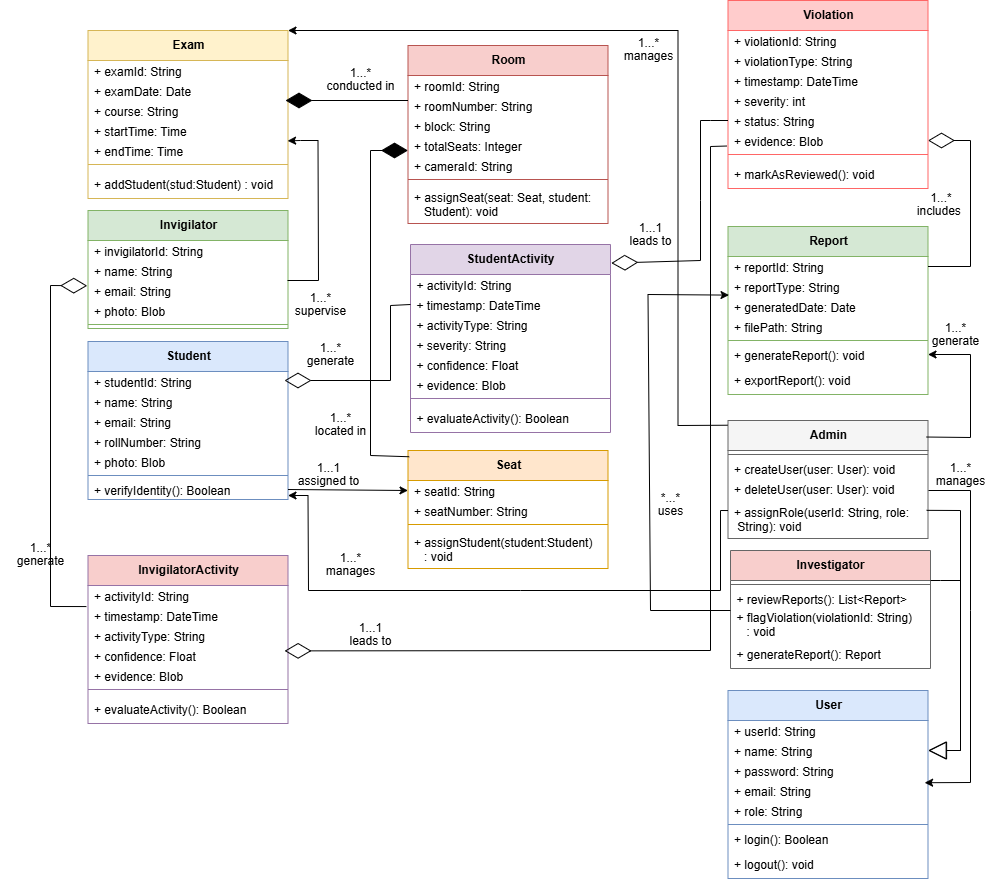
\includegraphics[width=\textwidth]{sections/class-diagram.png}
    \label{fig:class}
\end{figure}
\clearpage

\subsection{Activity Diagram}

The system's activity diagram illustrates the main processes and workflows:

\begin{figure}[H]
    \centering
    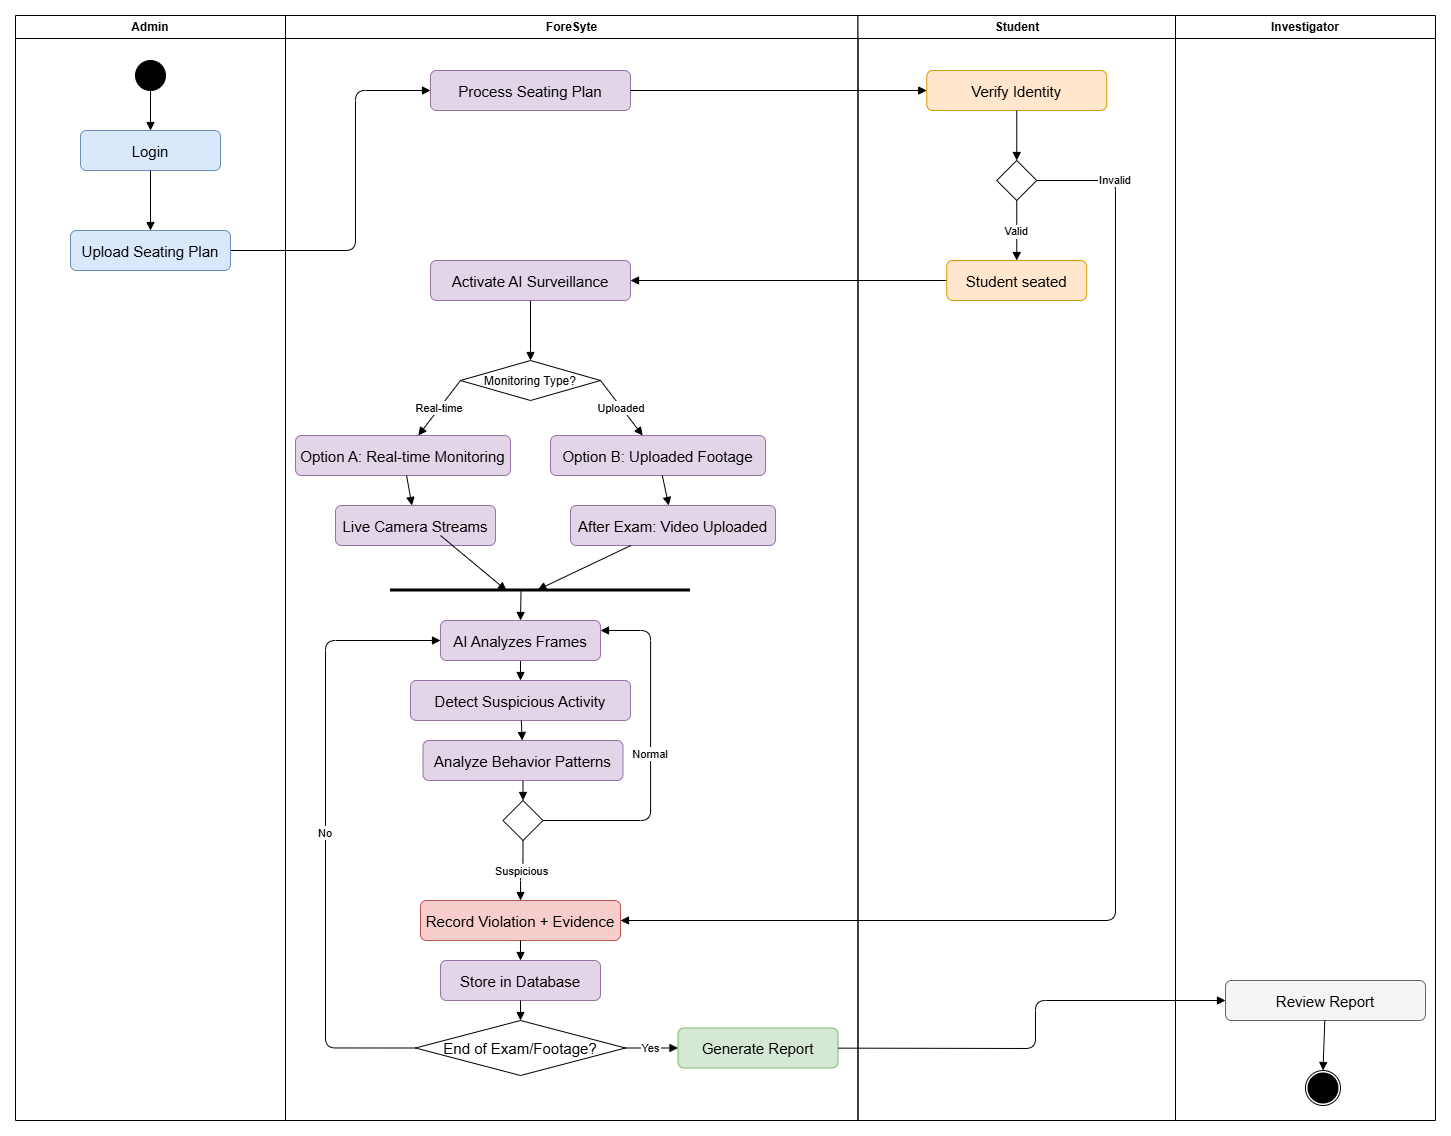
\includegraphics[width=0.95\textwidth,height=0.75\textheight,keepaspectratio]{sections/activity.png}
    \caption{ForeSyte Activity Diagram}
    \label{fig:activity}
\end{figure}
\FloatBarrier

% ------------------------
\subsection{System Sequence Diagram}

Figure~\ref{fig:ssd-foresyte} illustrates the high-level System Sequence Diagram (SSD) for ForeSyte. 
It depicts the main interactions between external actors (Students, Invigilators, Administrators, and the Discipline Committee) 
and the ForeSyte AI System across the examination workflow.  
This diagram provides an overview of how user actions trigger system processes such as attendance tagging, 
cheating detection, invigilator monitoring, and report generation.

\begin{figure}[H]
    \centering
    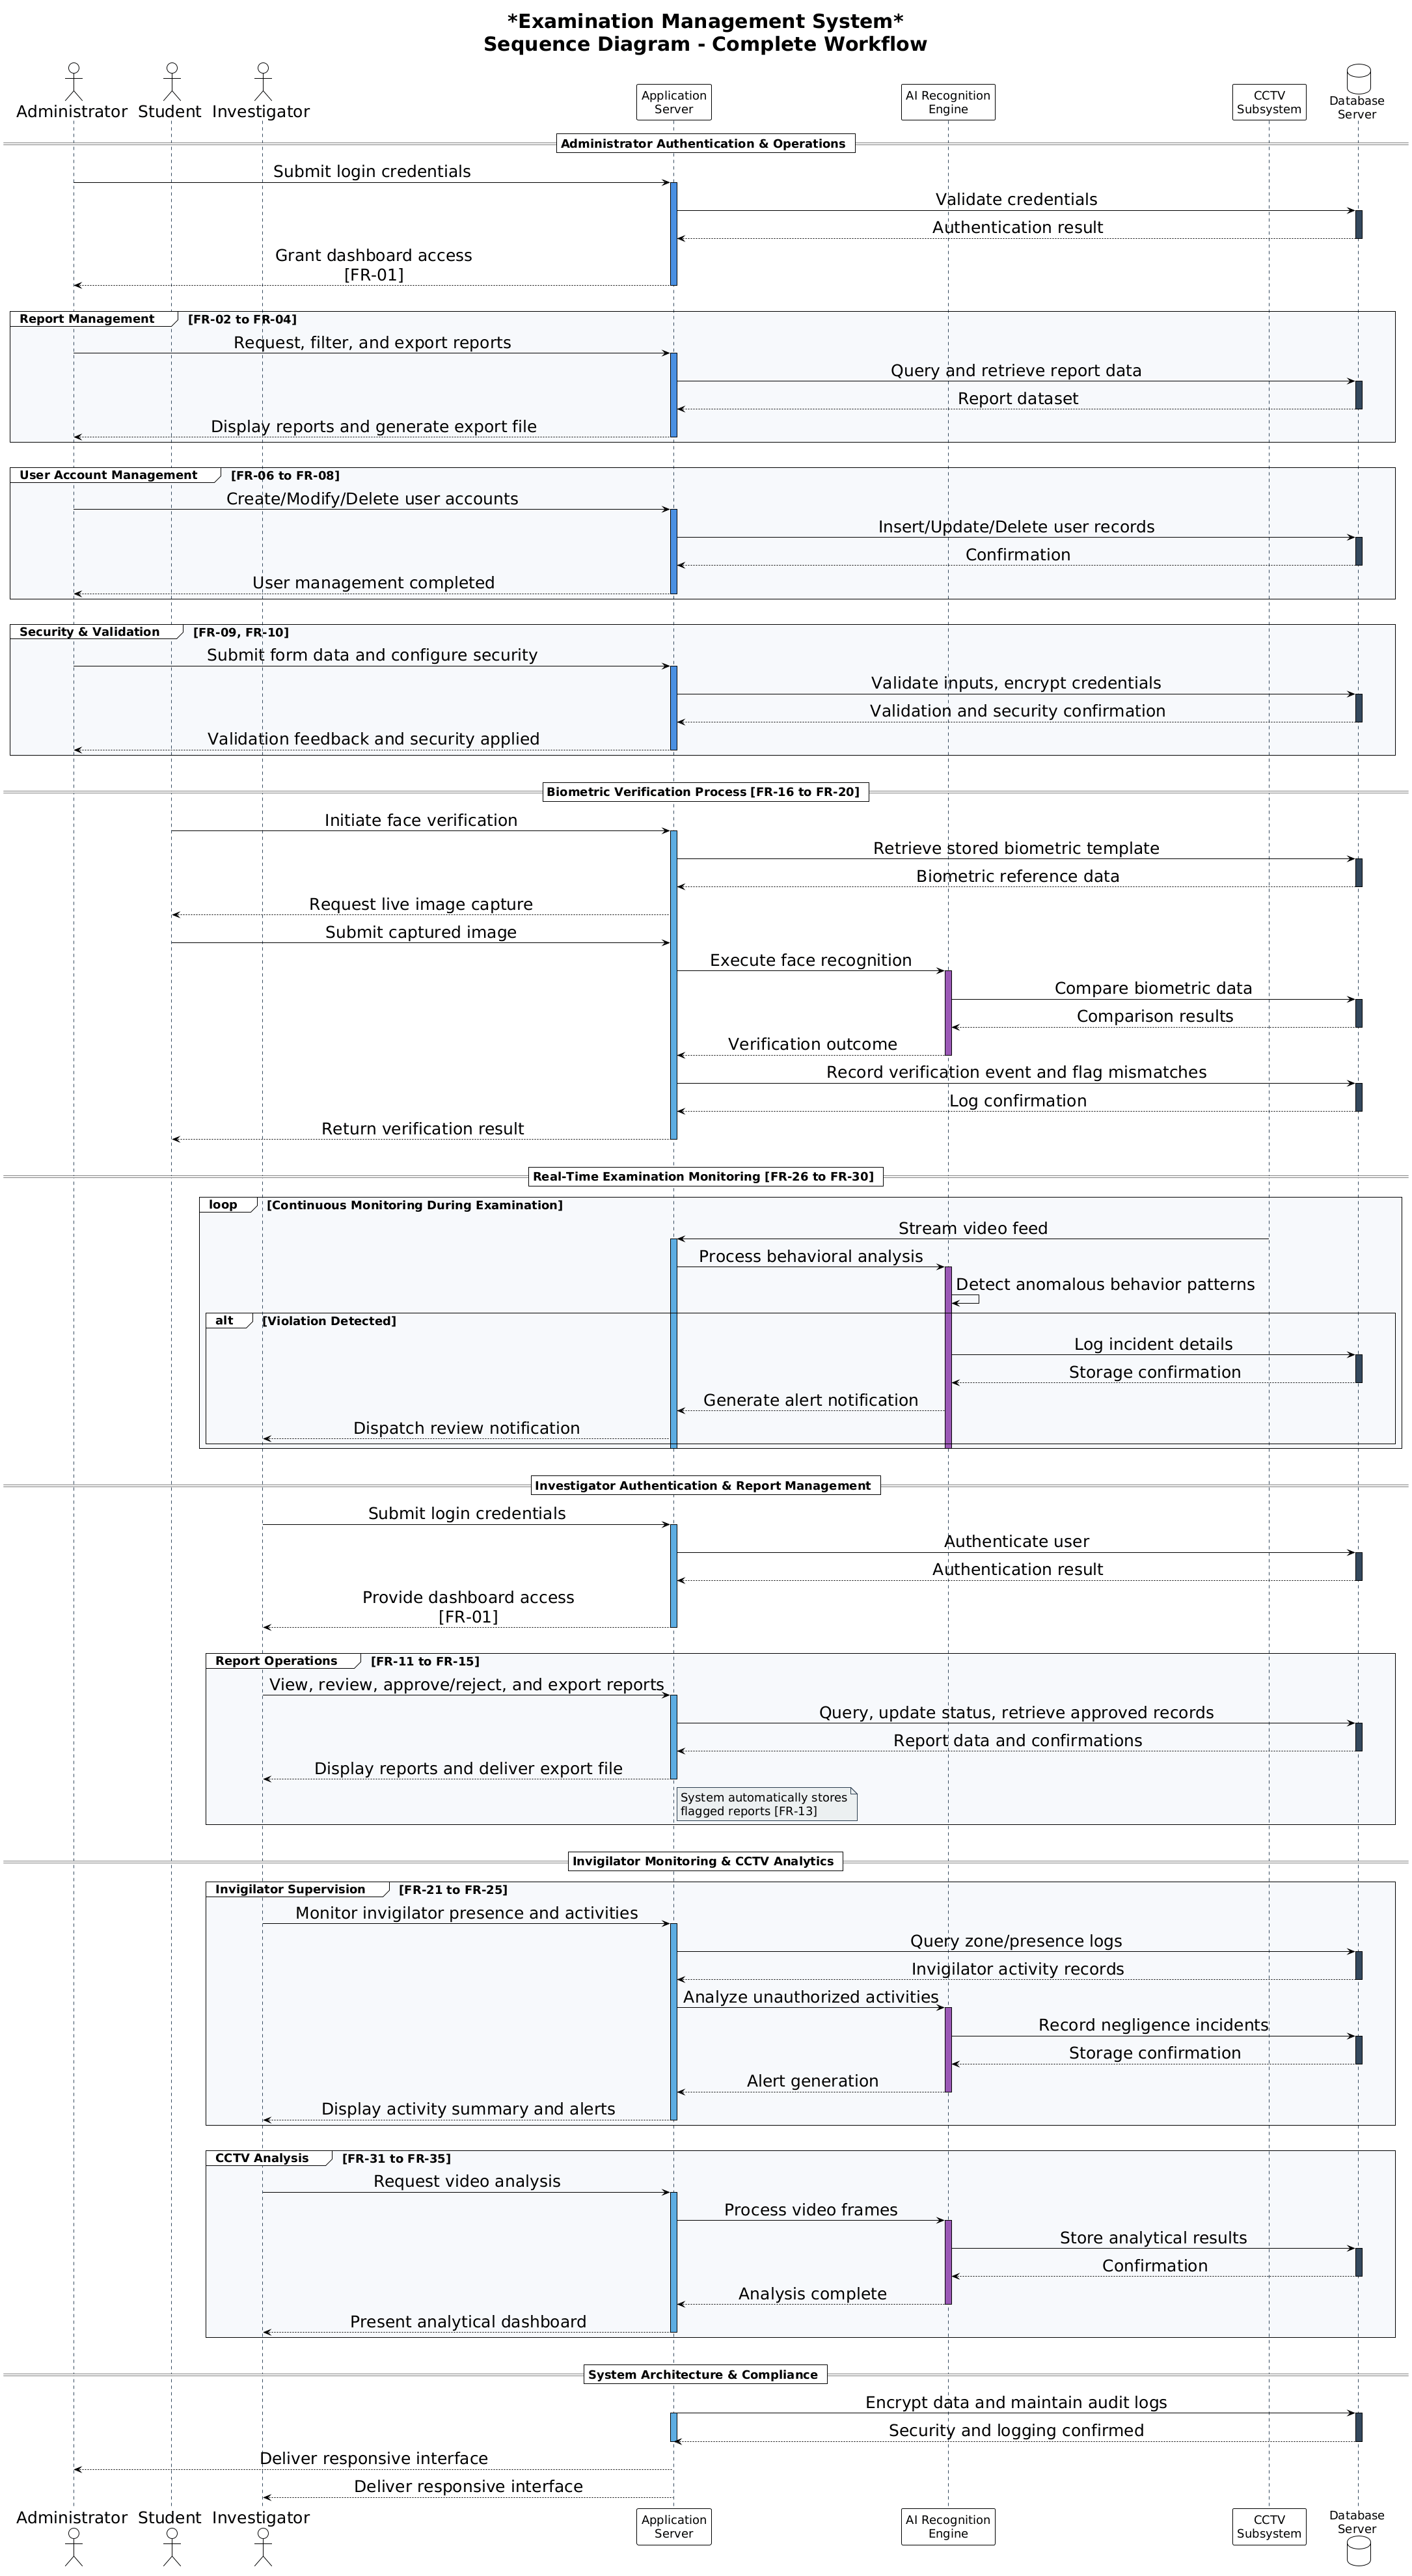
\includegraphics[width=\textwidth,height=0.85\textheight,keepaspectratio]{sections/ssd.png}
    \caption{System Sequence Diagram for ForeSyte}
    \label{fig:ssd-foresyte}
\end{figure}

% ------------------------
\subsection{Sequence Diagrams}
\vspace*{-0.5em}
This section presents the sequence diagrams for all identified use cases (UC-01 to UC-07). 
Each diagram illustrates the dynamic interaction between actors, the ForeSyte AI System, 
and domain entities.

% ---------- UC-01 ----------
\begin{figure}[H]
    \centering
    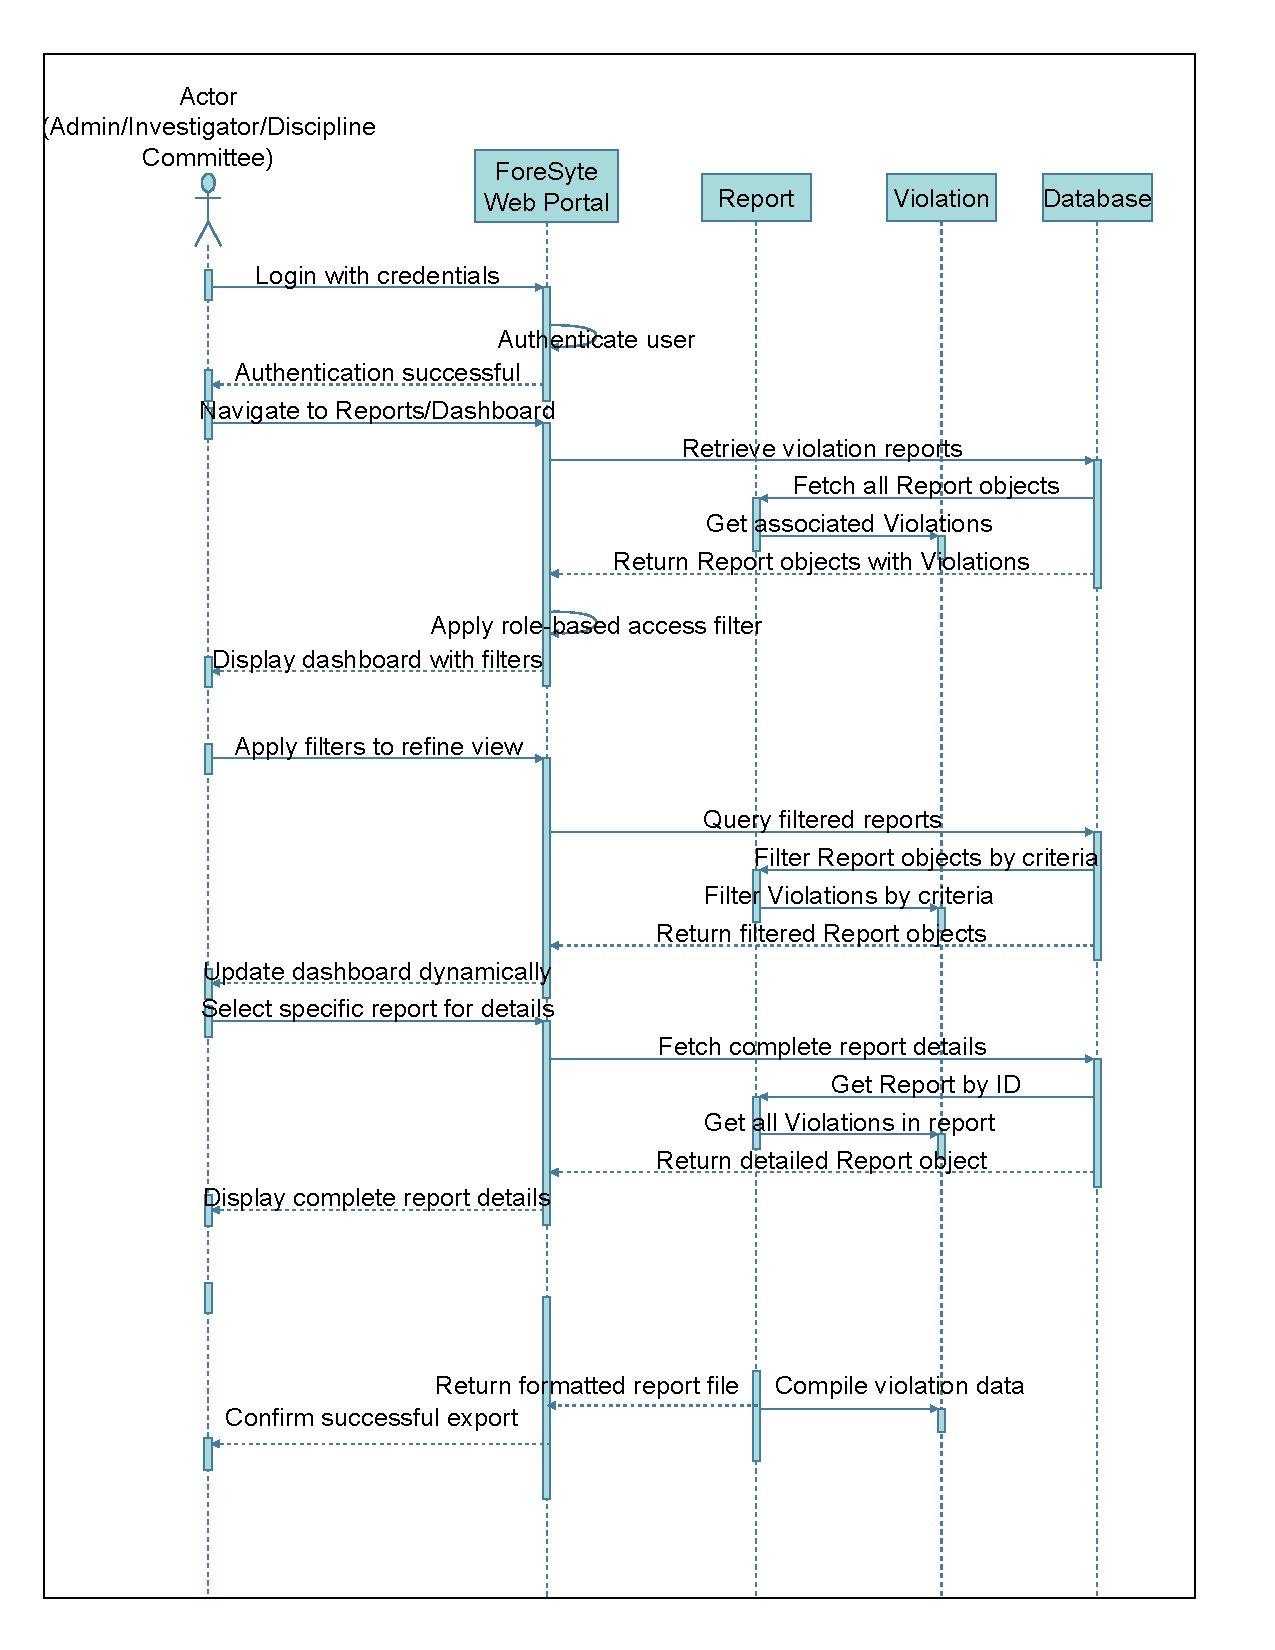
\includegraphics[width=\textwidth,height=\textheight,keepaspectratio]{sections/uc01.pdf}
    \caption{Sequence Diagram for UC-01: View and Manage Reports/Dashboard}
    \label{fig:uc01}
\end{figure}
\clearpage

% ---------- UC-02 ----------
\begin{figure}[p]
    \centering
    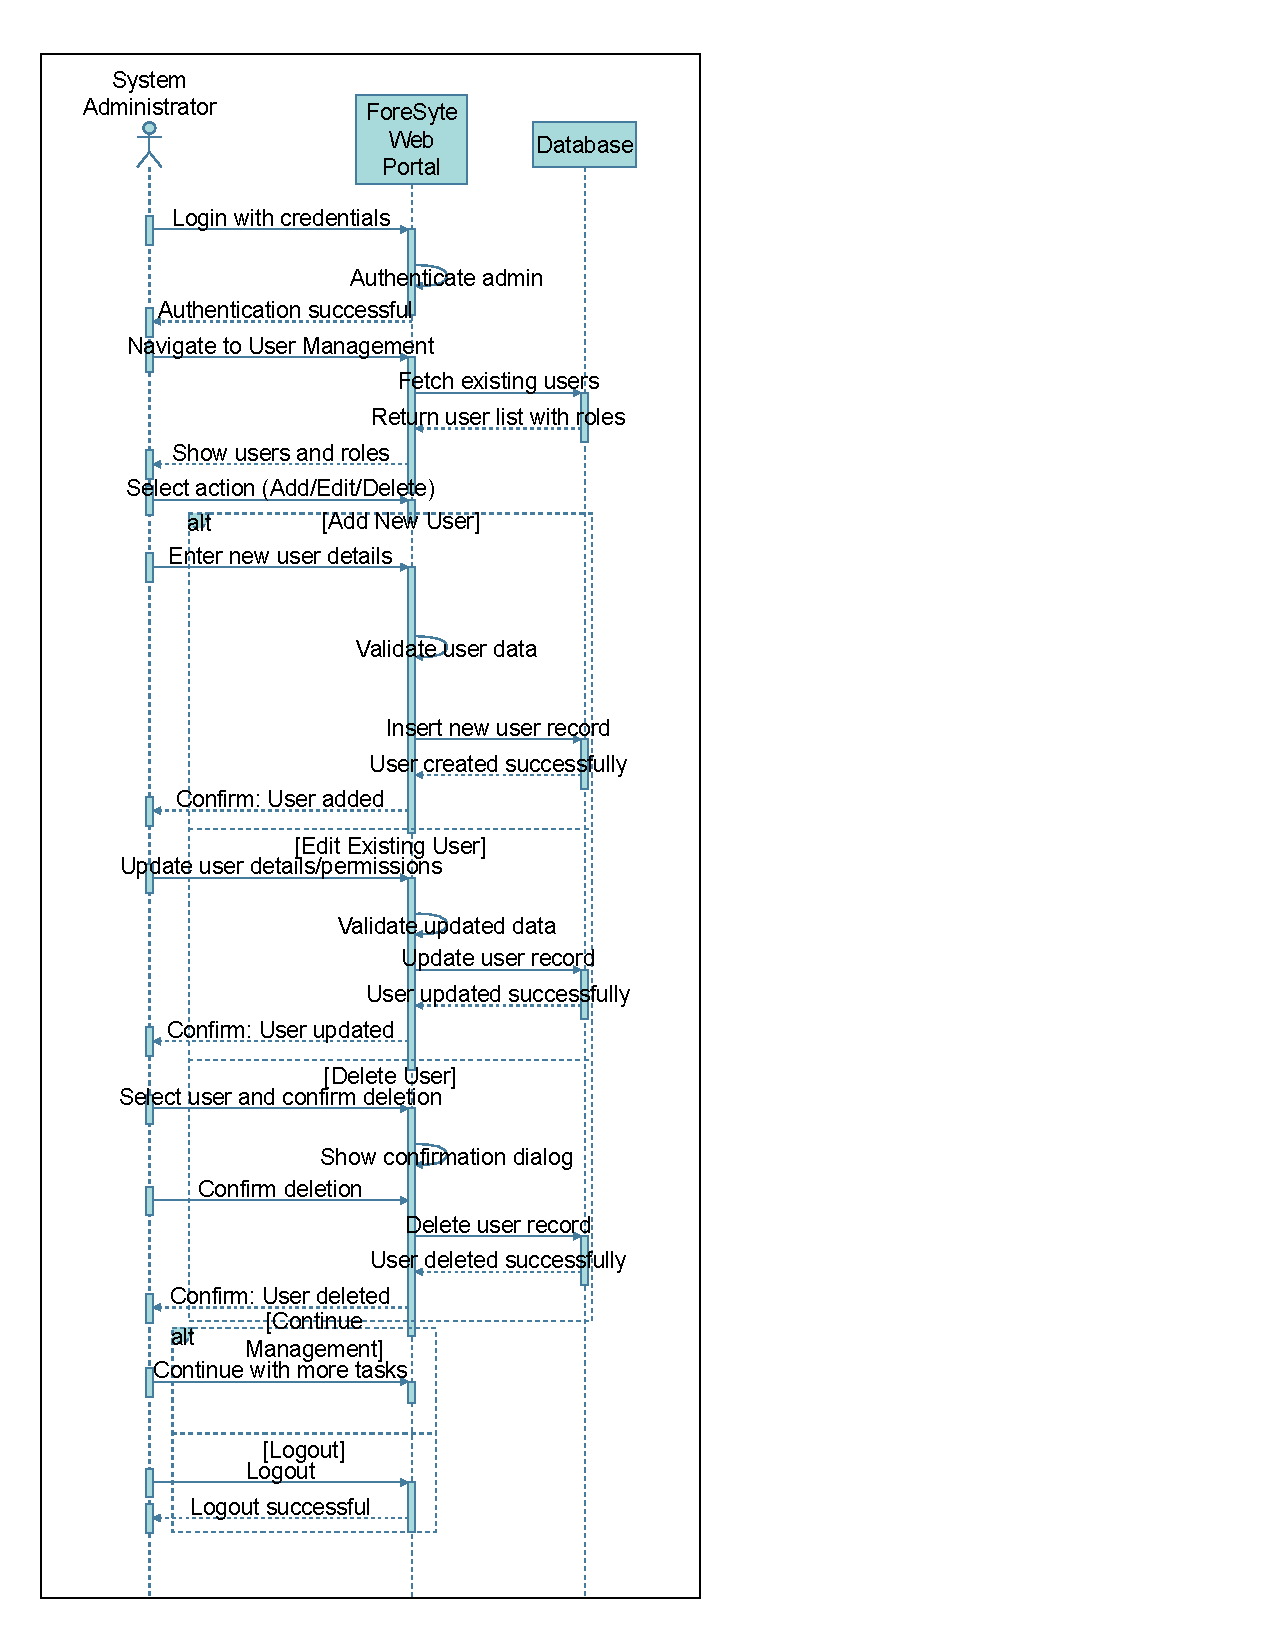
\includegraphics[width=\textwidth,height=\textheight,keepaspectratio]{sections/uc02.pdf}
    \caption{Sequence Diagram for UC-02: Manage User Profiles}
    \label{fig:uc02}
\end{figure}
\clearpage

% ---------- UC-03 ----------
\begin{figure}[p]
    \centering
    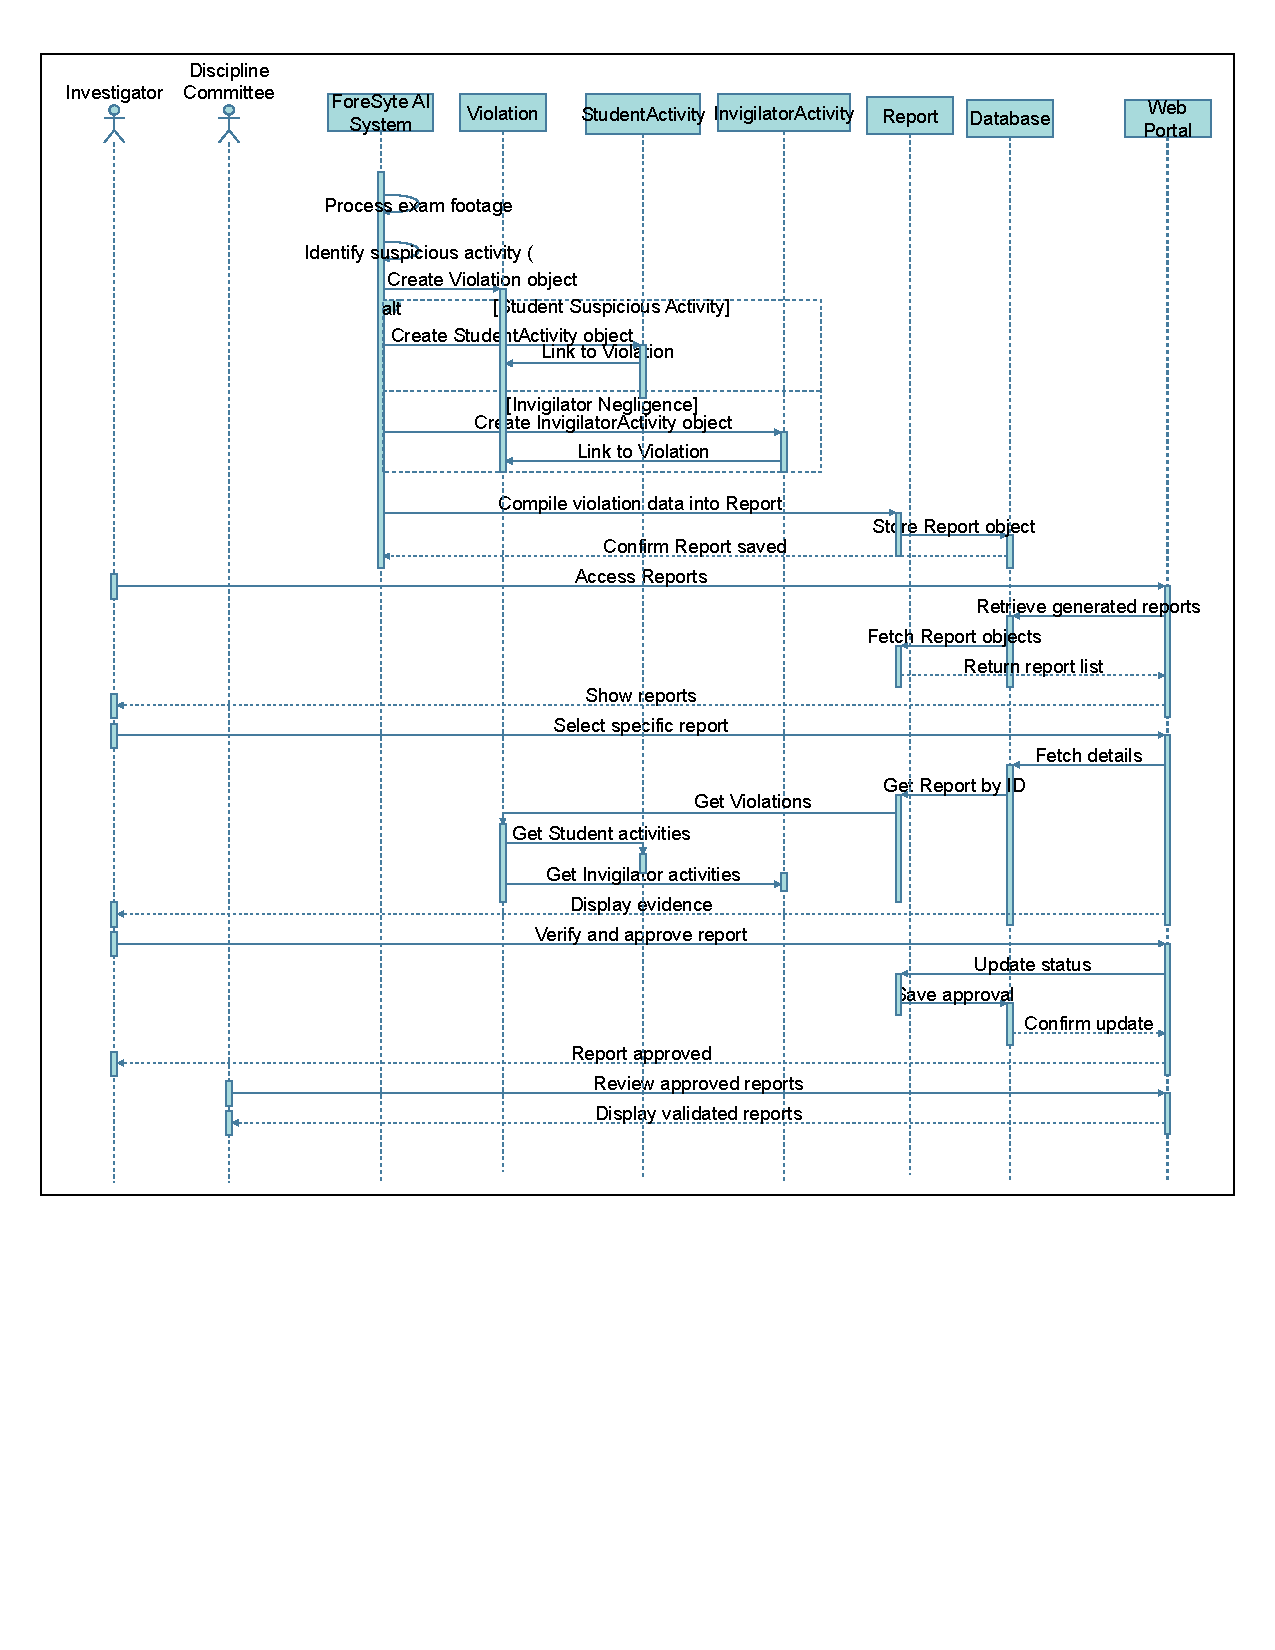
\includegraphics[width=\textwidth,height=\textheight,keepaspectratio]{sections/uc03.pdf}
    \caption{Sequence Diagram for UC-03: Generate Detection Reports}
    \label{fig:uc03}
\end{figure}
\clearpage
% ---------- UC-04 ----------
\begin{figure}[p]
    \centering
    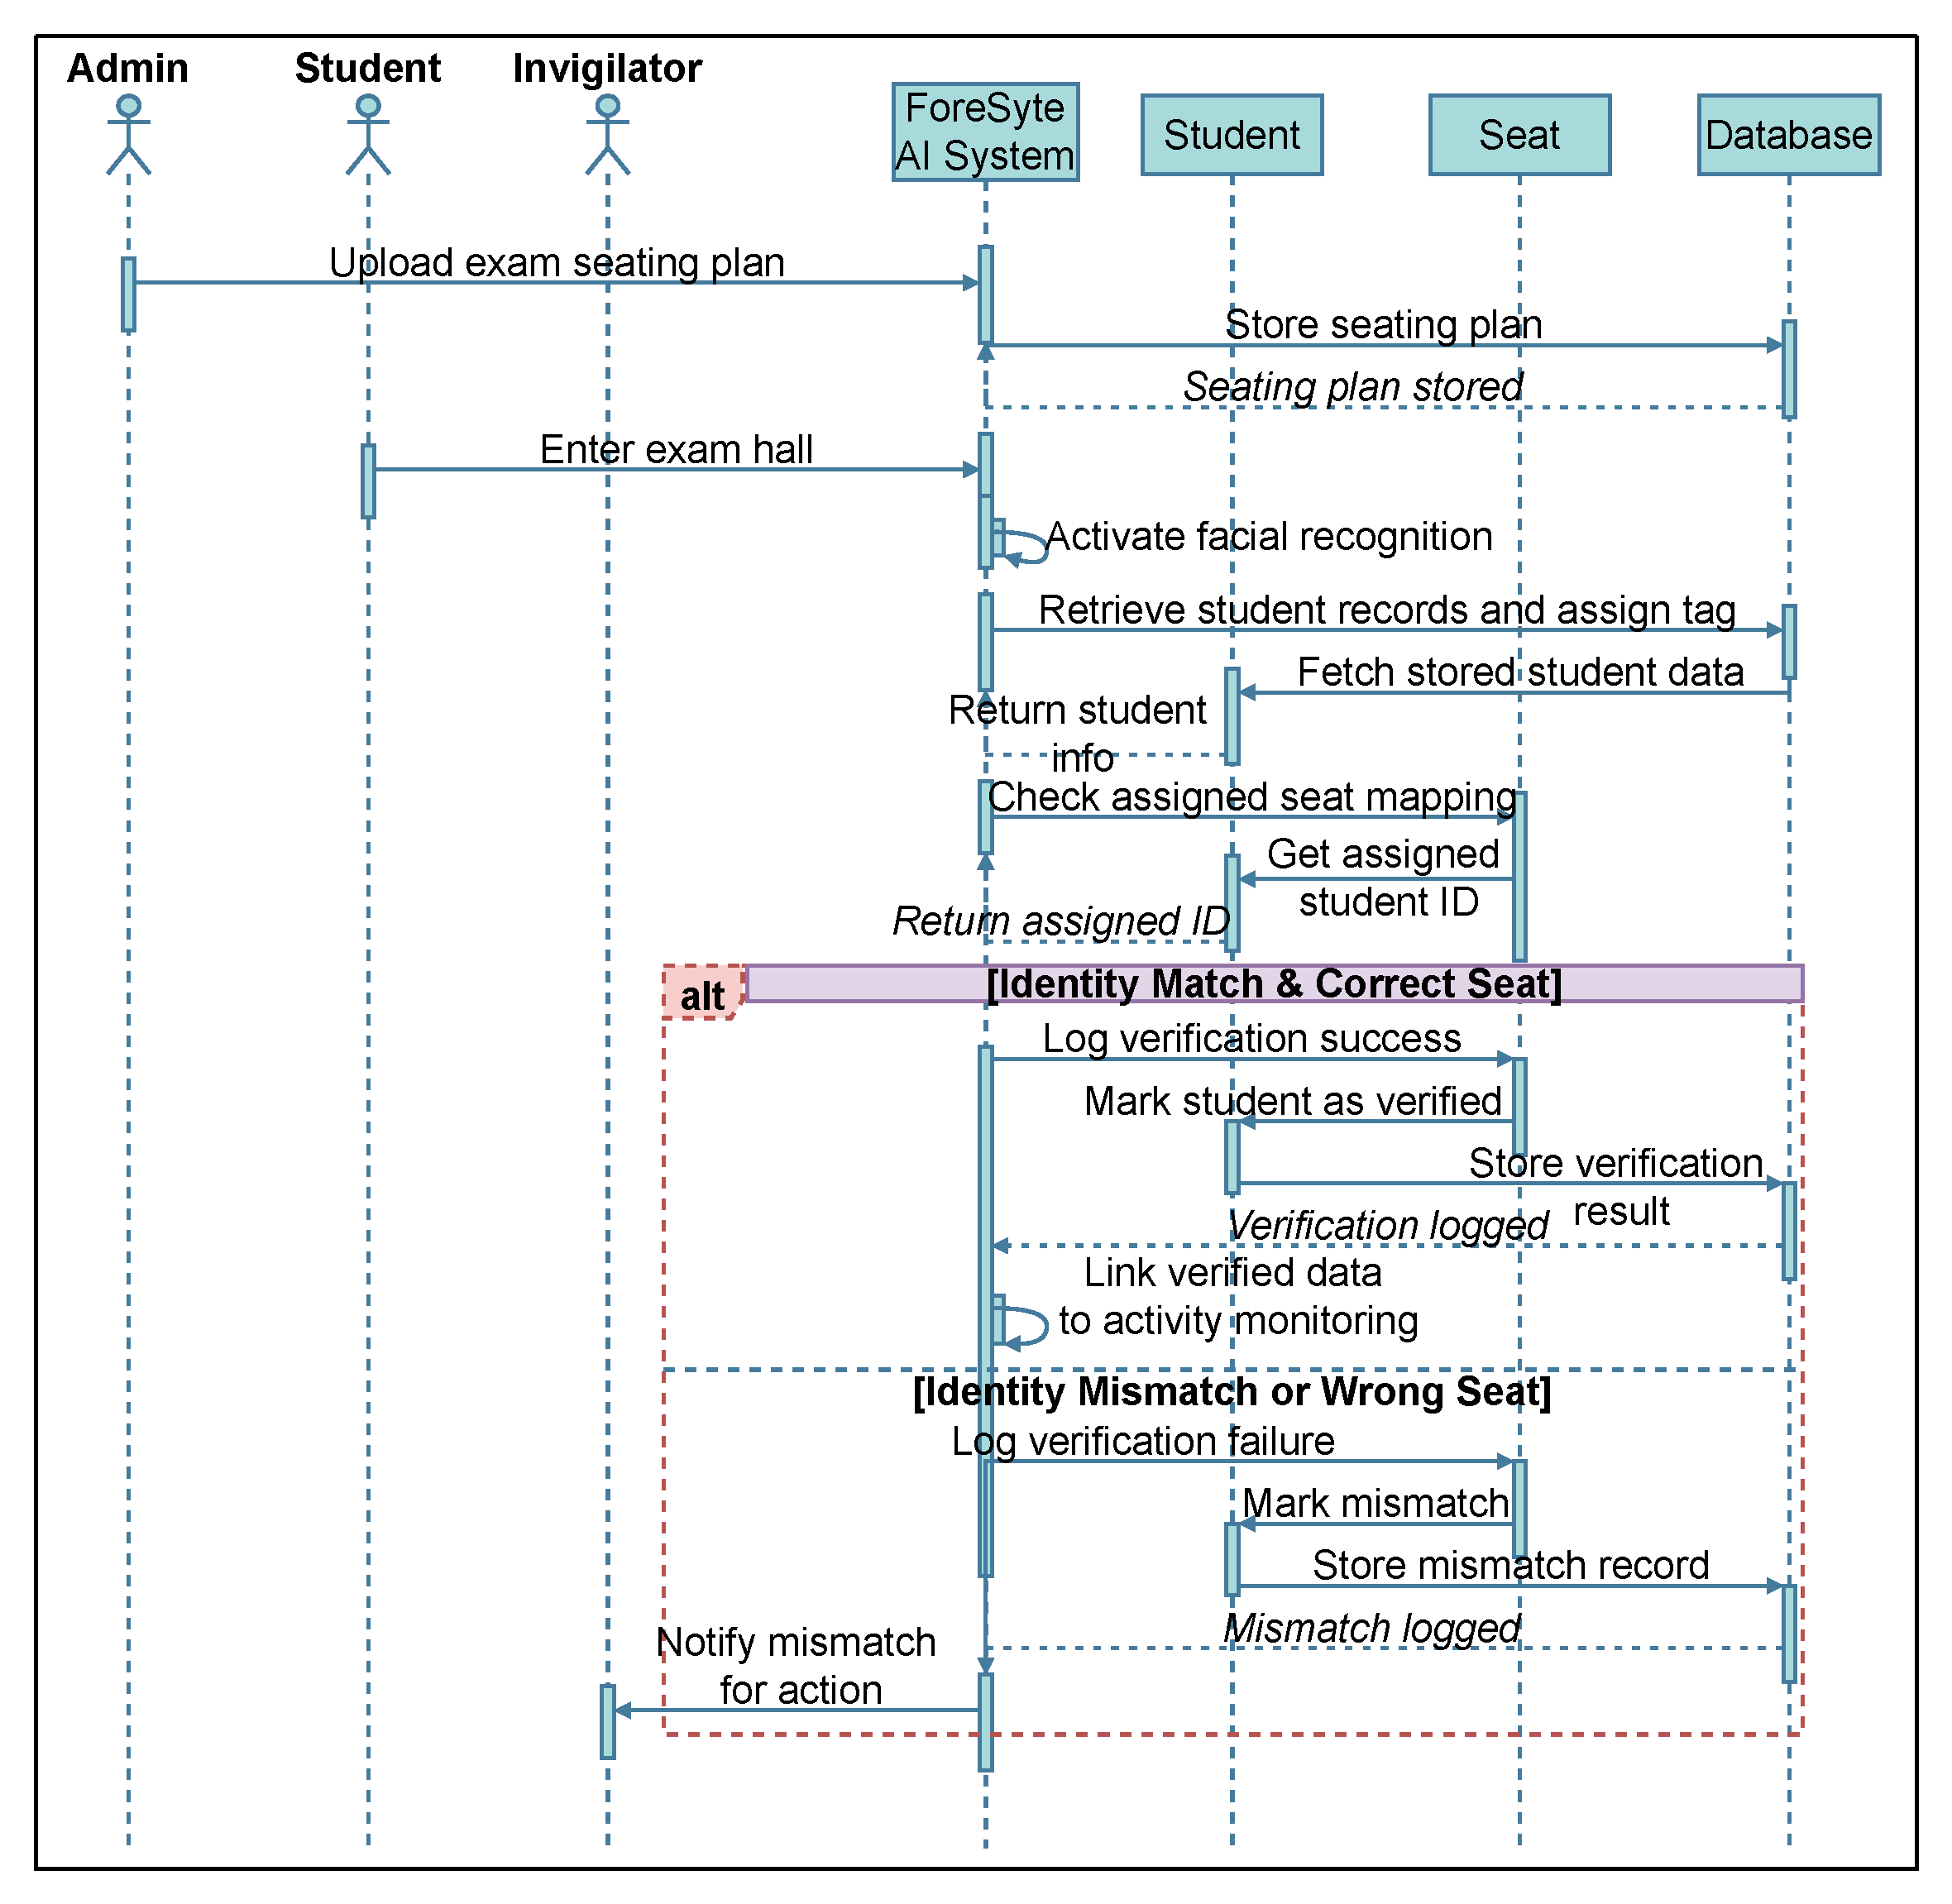
\includegraphics[width=\textwidth,height=\textheight,keepaspectratio]{sections/uc04.pdf}
    \caption{Sequence Diagram for UC-04: Verify Student Identity \& Seat Mapping}
    \label{fig:uc04}
\end{figure}
\clearpage

% ---------- UC-05 ----------
\begin{figure}[p]
    \centering
    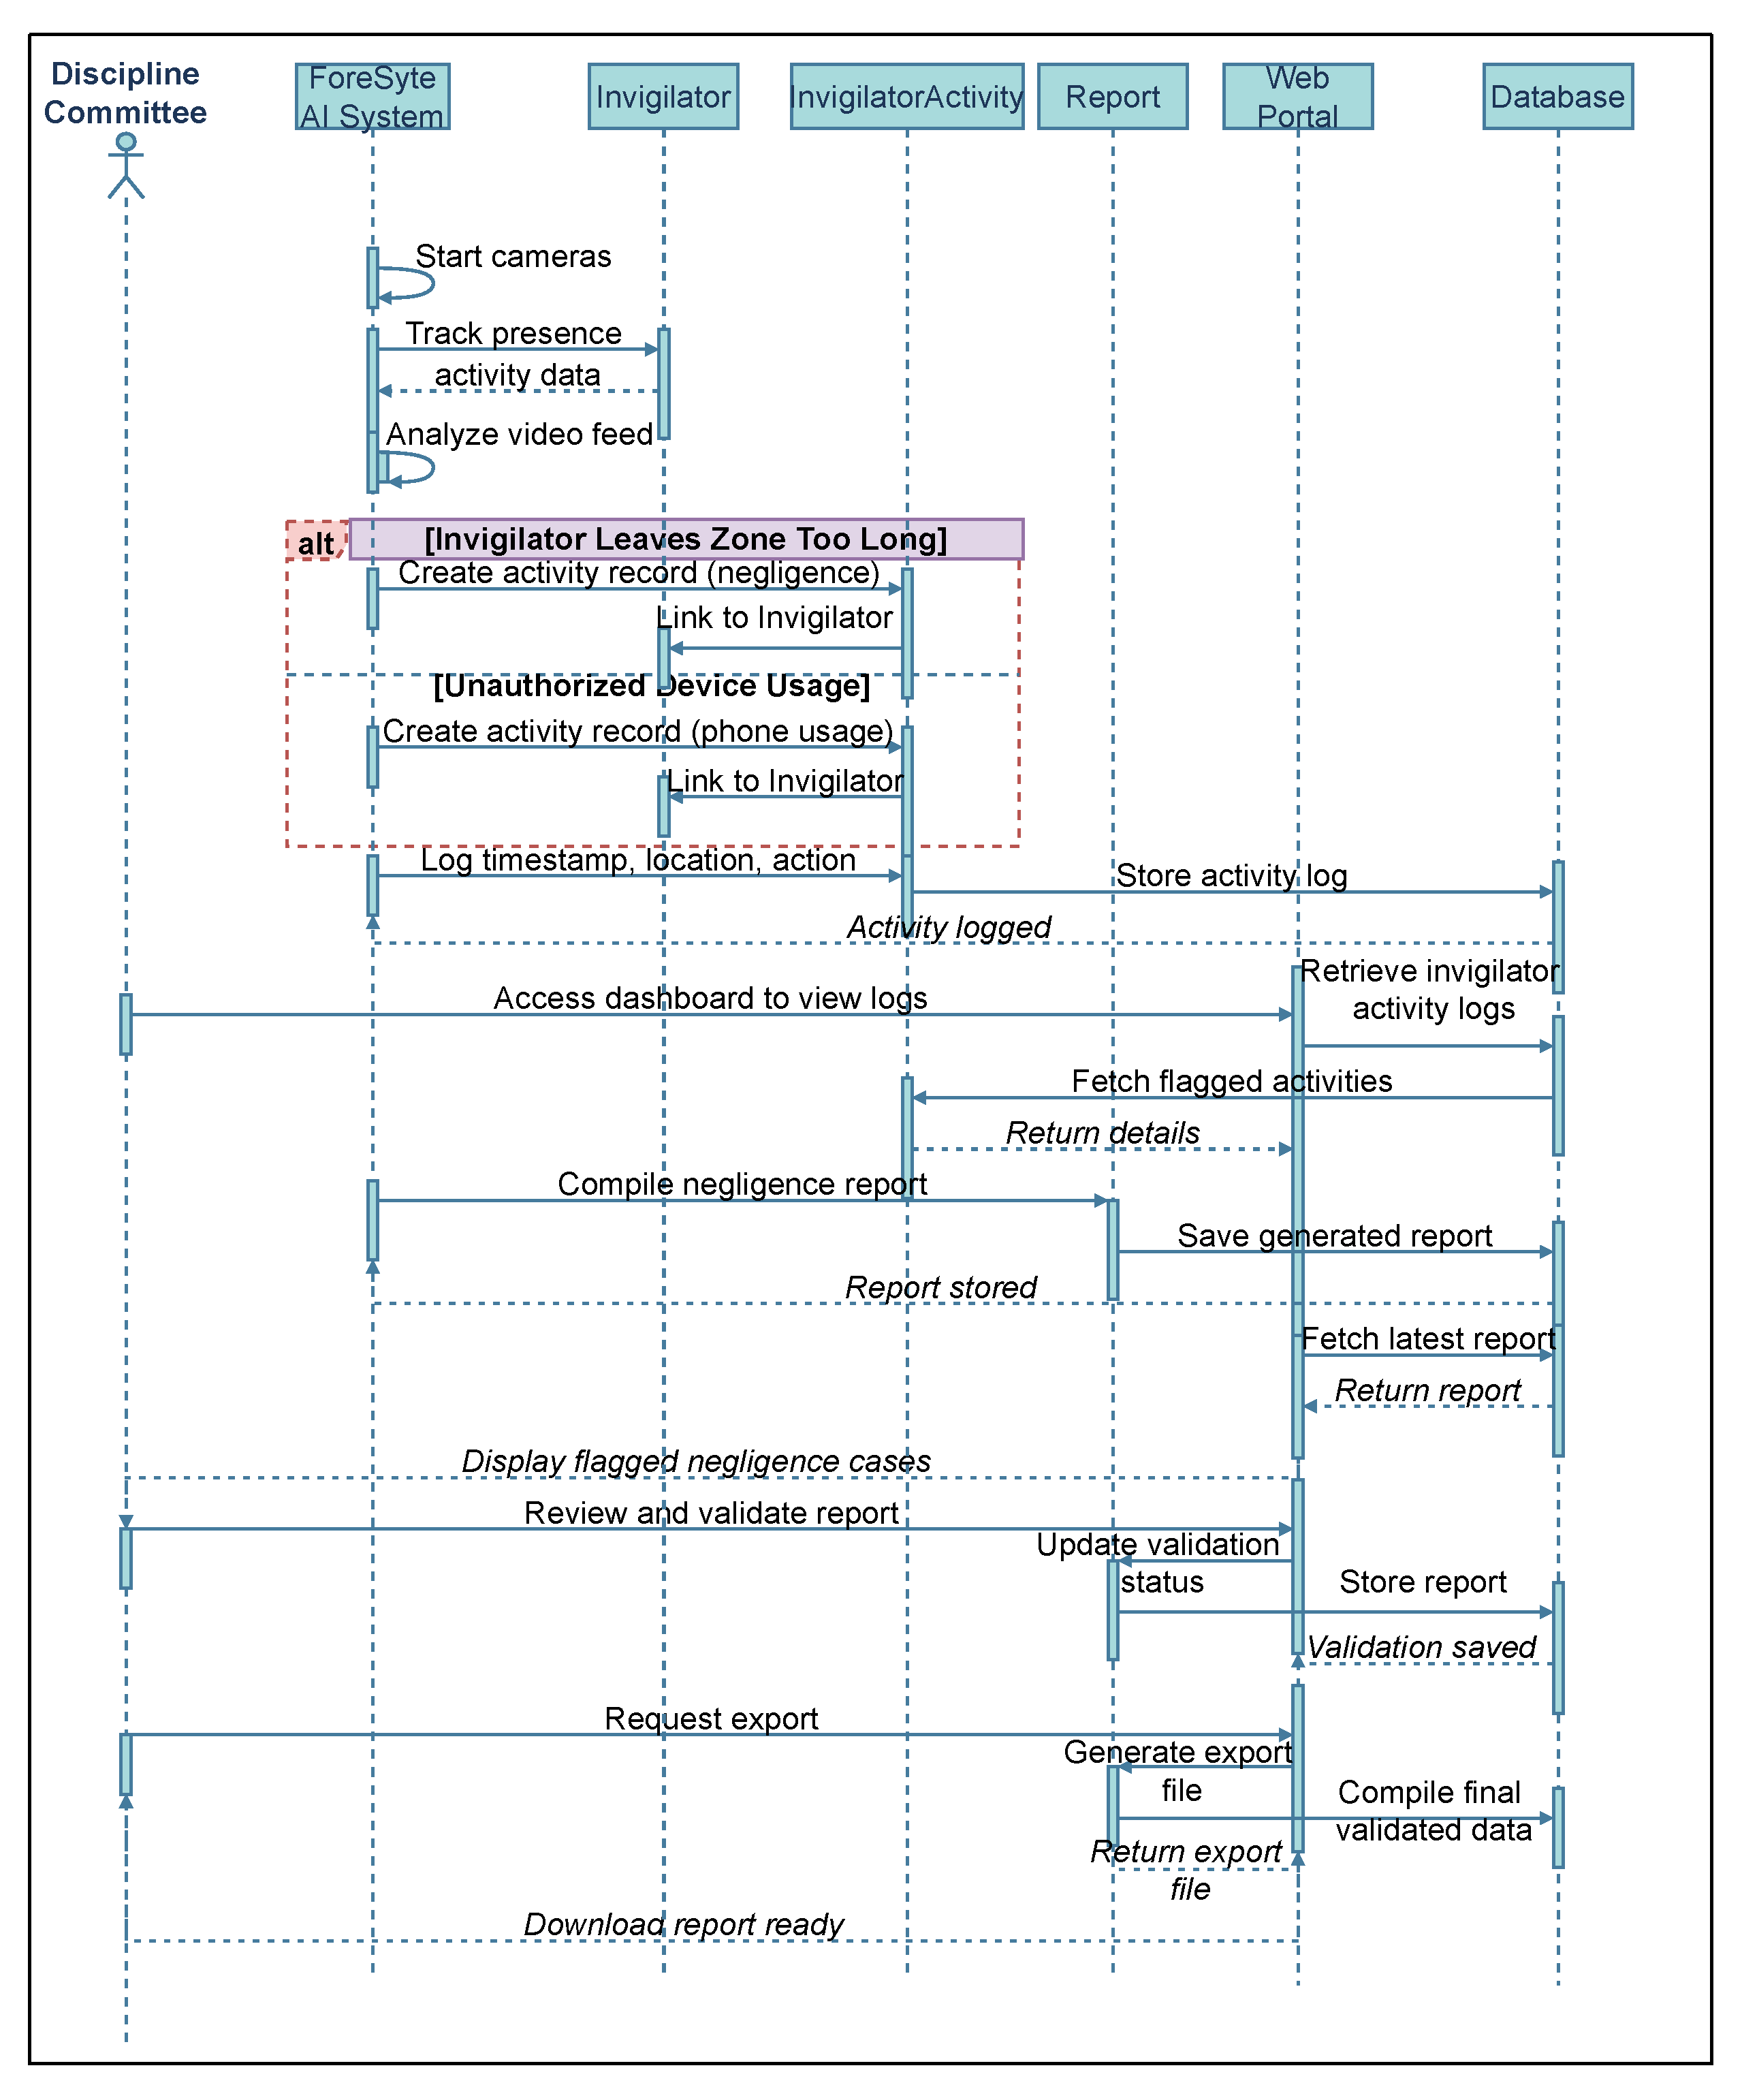
\includegraphics[width=\textwidth,height=\textheight,keepaspectratio]{sections/uc05.pdf}
    \caption{Sequence Diagram for UC-05: Monitor Invigilator Activity}
    \label{fig:uc05}
\end{figure}
\clearpage


% ---------- UC-06 ----------
\begin{figure}[p]
    \centering
 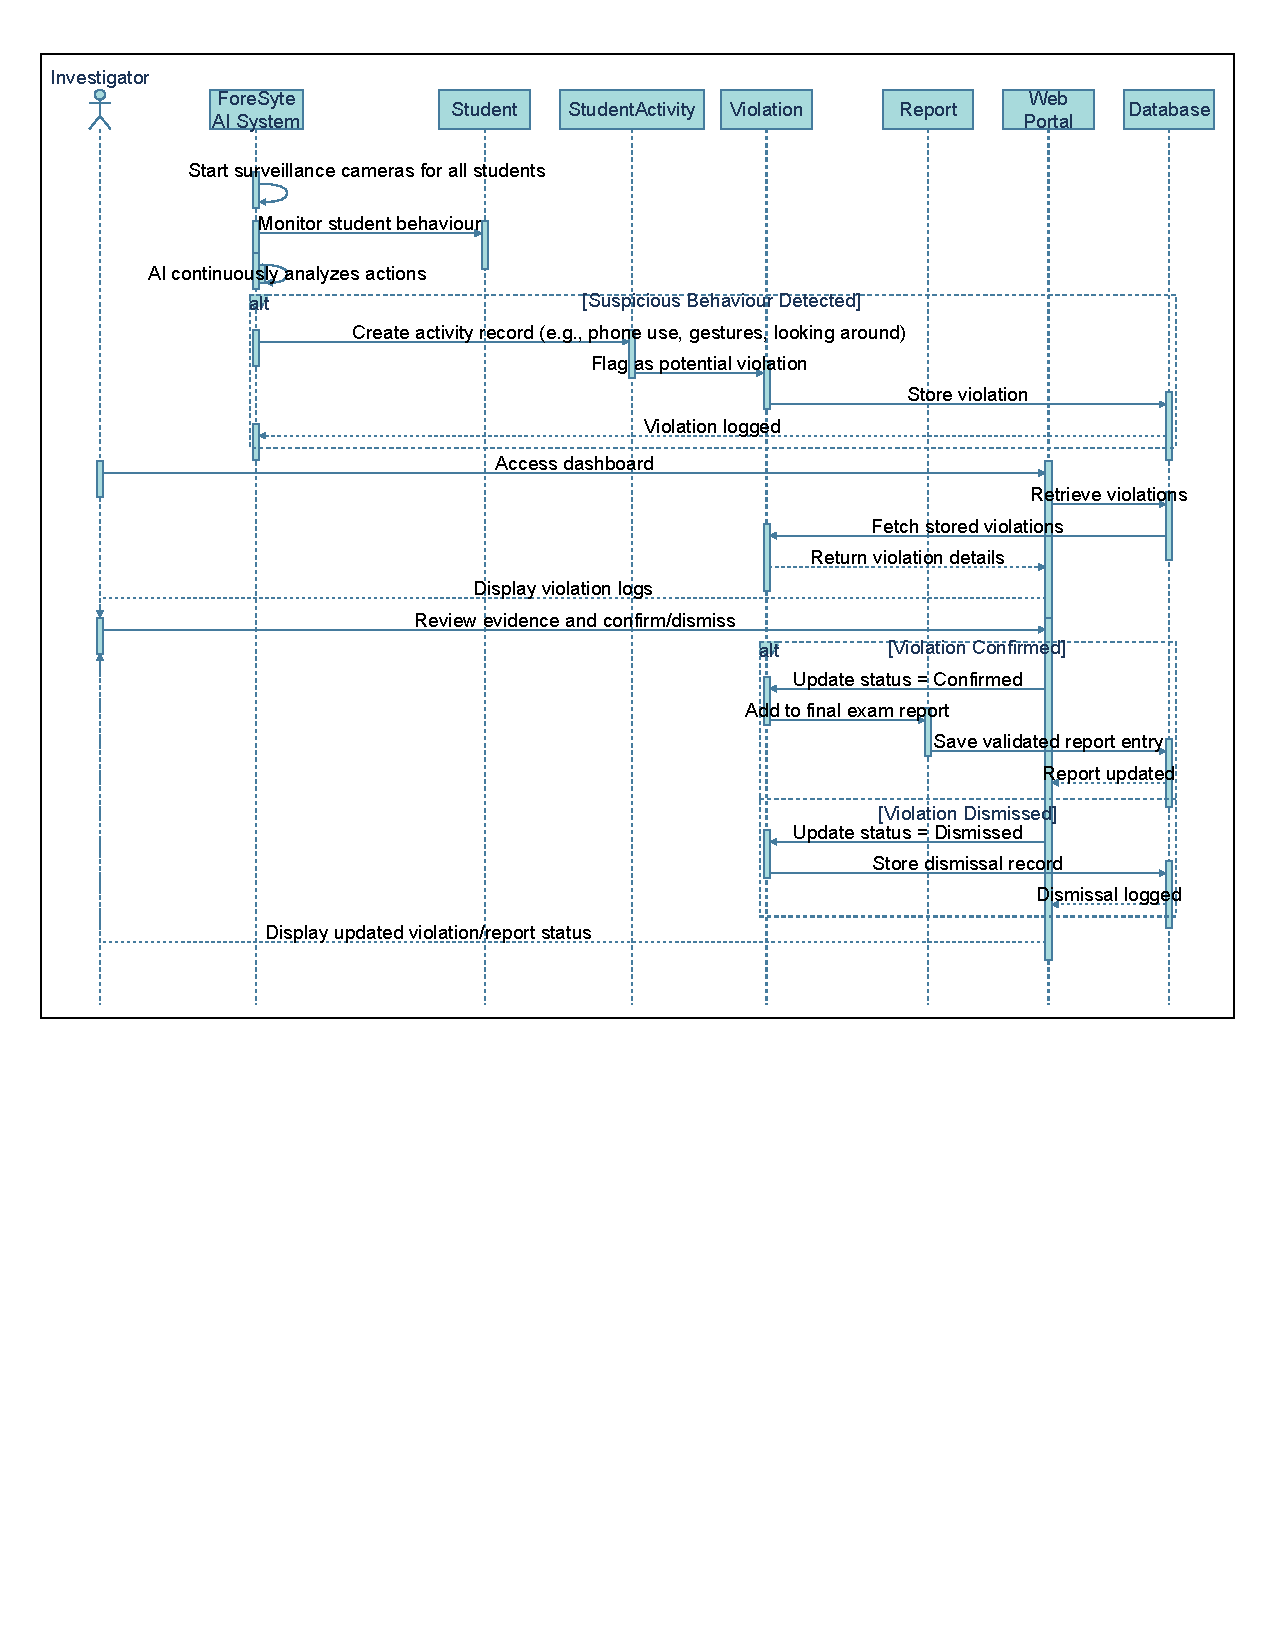
\includegraphics[width=\textwidth,height=\textheight,keepaspectratio]{sections/uc06.pdf}

    \caption{Sequence Diagram for UC-06: Monitor Student Behaviour}
    \label{fig:uc06}
\end{figure}
\clearpage

% ---------- UC-07 ----------
\begin{figure}[p]
    \centering
 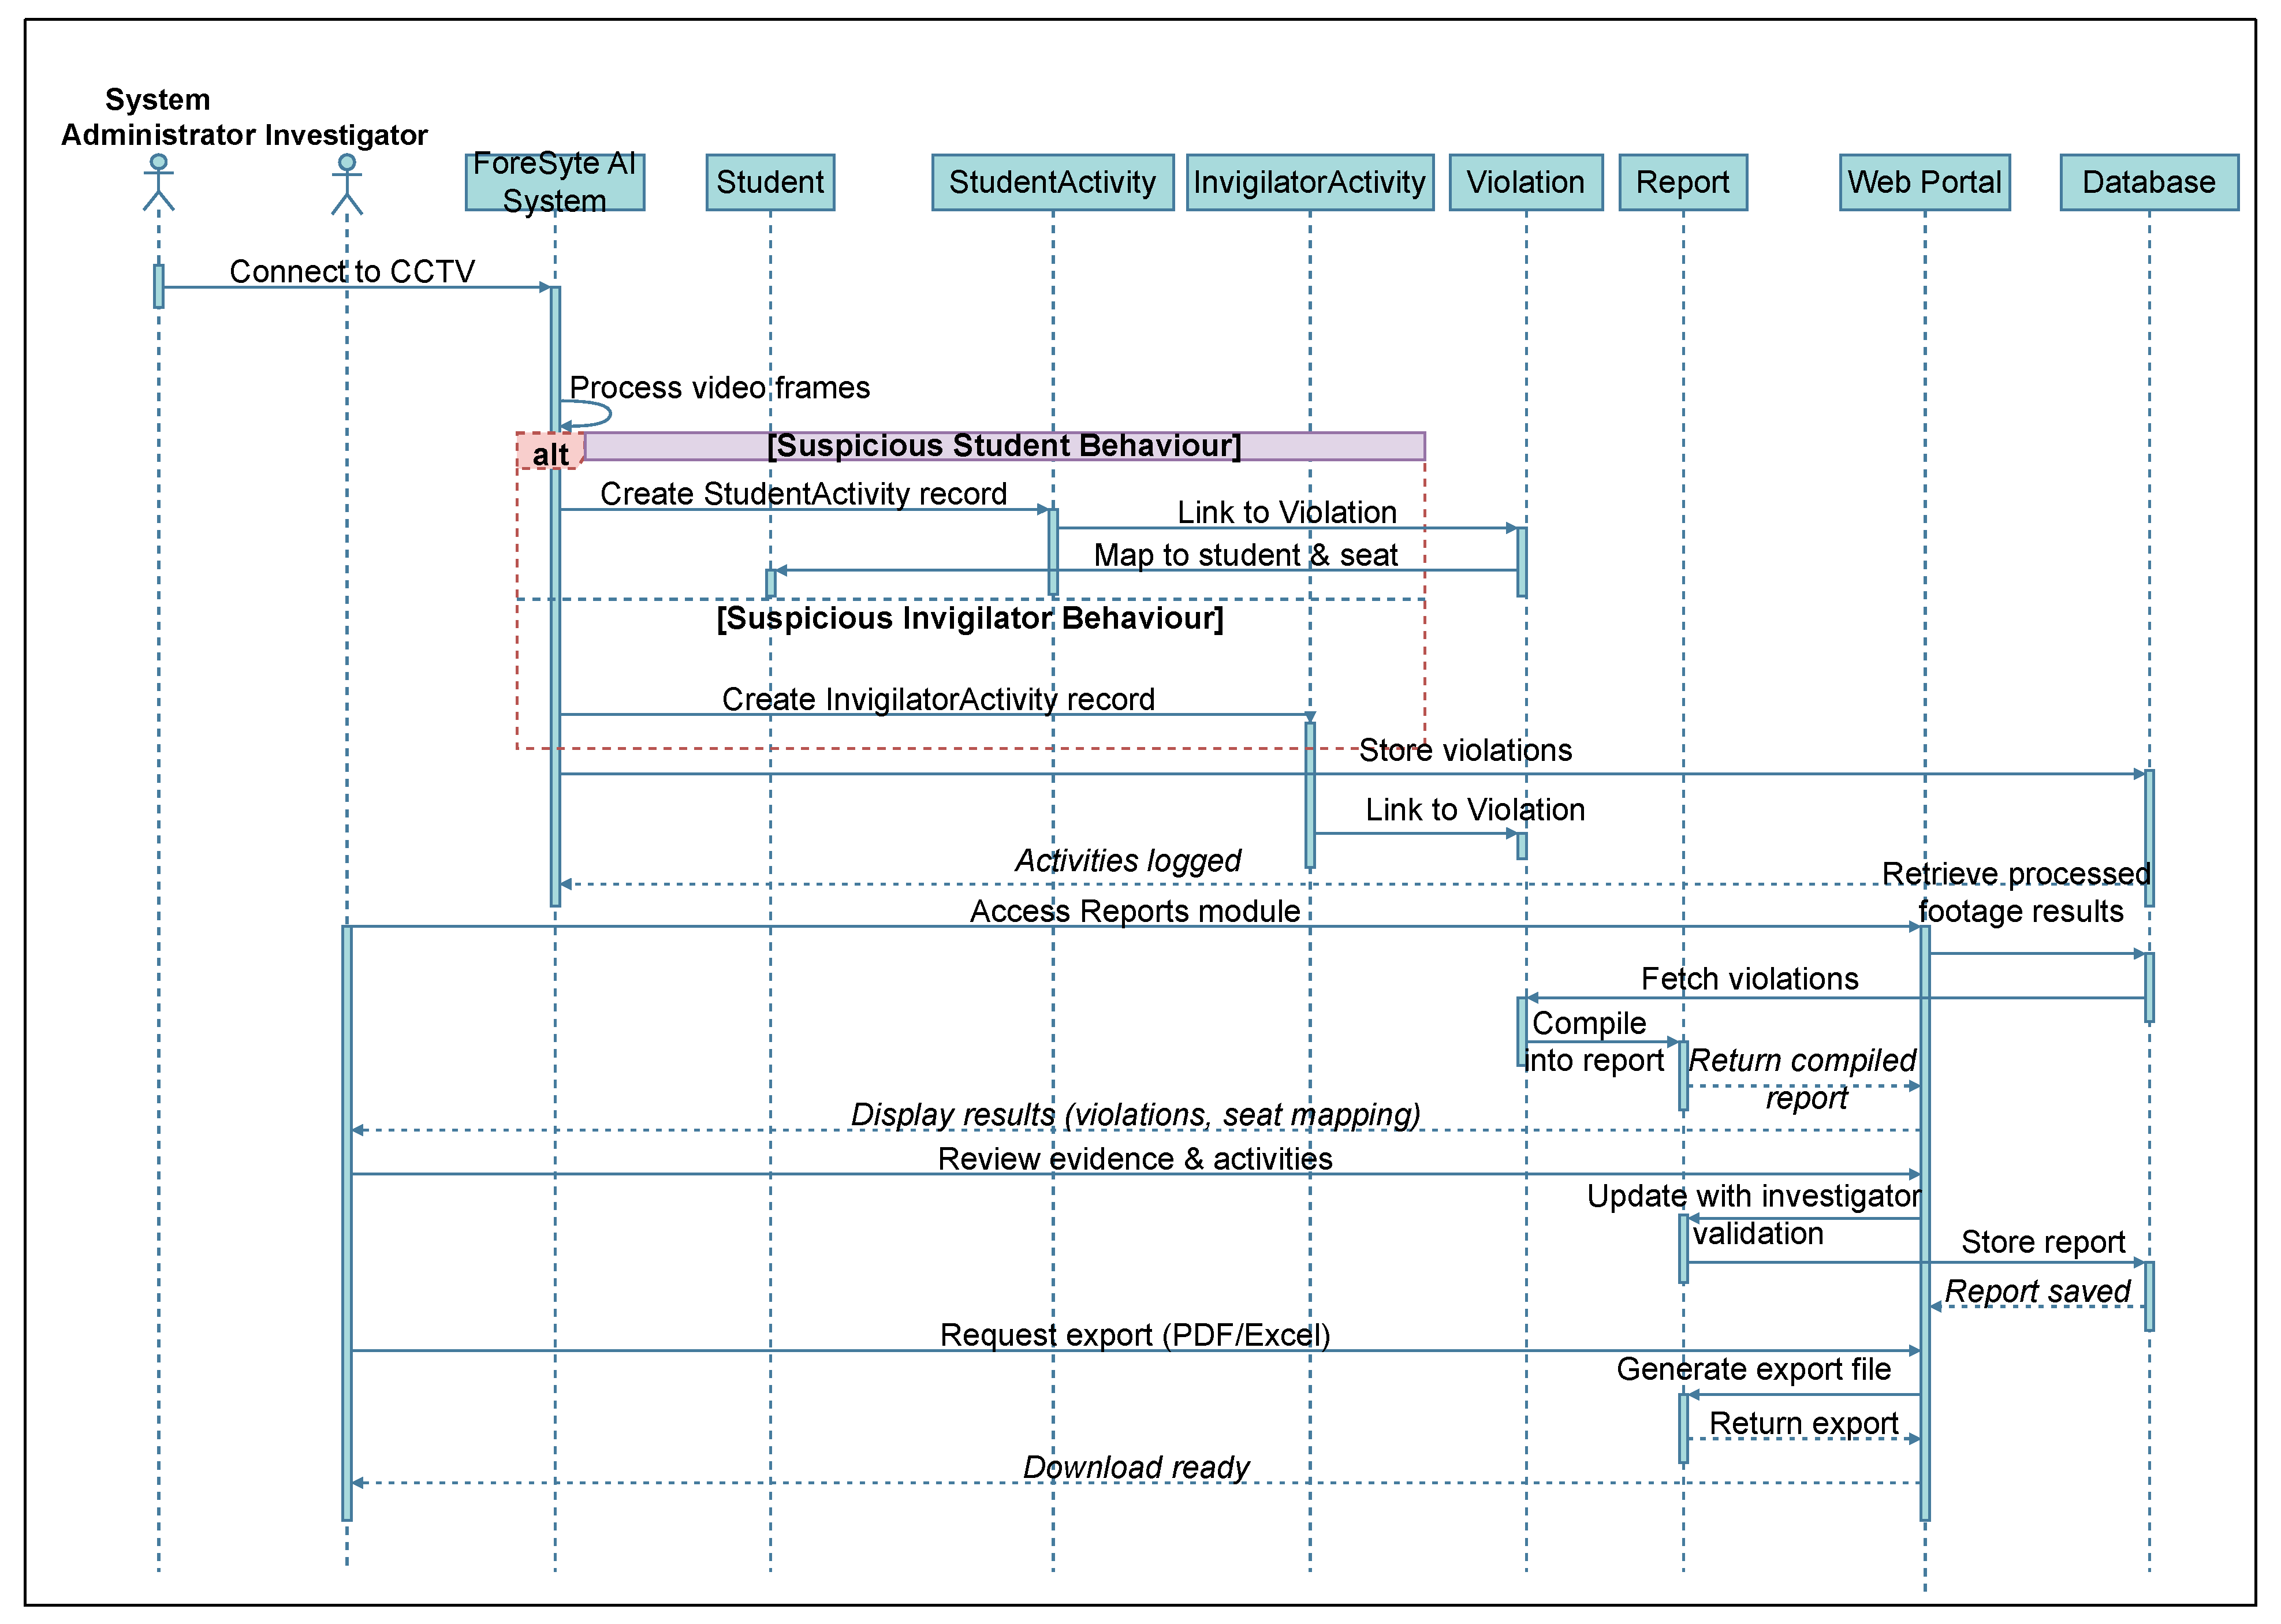
\includegraphics[width=\textwidth,height=\textheight,keepaspectratio]{sections/uc07.pdf}
    \caption{Sequence Diagram for UC-07: Process Exam Footage (Live/Recorded)}
    \label{fig:uc07}
\end{figure}
\clearpage

\subsection{State Transition Diagram}

\begin{figure}[H]
    \centering
    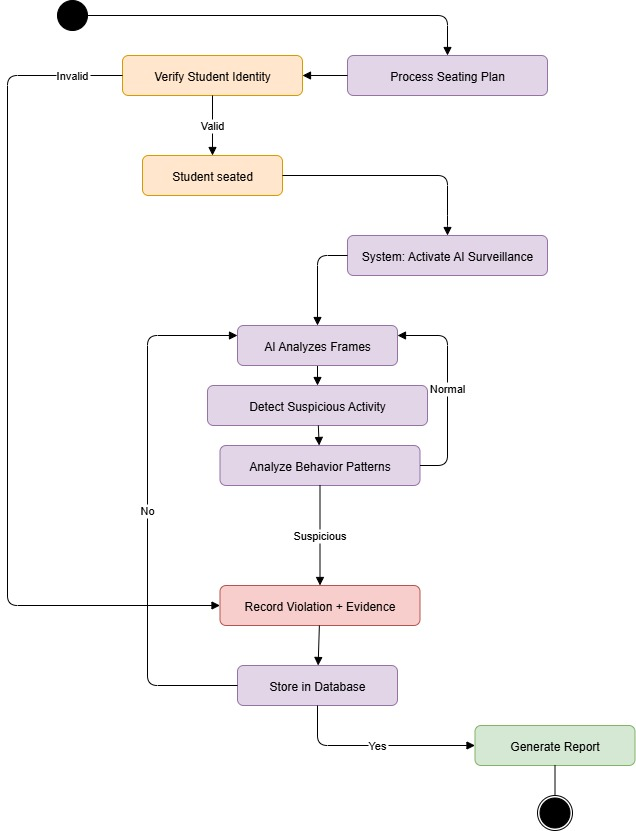
\includegraphics[width=\textwidth]{sections/std.jpg}
    \caption{State Transition Diagram}
    \label{fig:state-diagram}
\end{figure}
\FloatBarrier
This model collectively provide a comprehensive view of the ForeSyte system's architecture, ensuring clear understanding of system components, their interactions, and the overall system behavior throughout the examination monitoring process.





